\documentclass[12pt,a4paper]{article}
\usepackage[utf8]{inputenc}
\usepackage[croatian]{babel}
\usepackage[T1]{fontenc}
\usepackage{graphicx}
\usepackage{geometry}
\usepackage{setspace}
\usepackage{titlesec}
\usepackage{fancyhdr}
\usepackage{caption}
\hyphenpenalty=10000
\exhyphenpenalty=10000
\sloppy

% Postavke margina
\geometry{left=3cm,right=2.5cm,top=2.5cm,bottom=2.5cm}

% Prored 1.5
\onehalfspacing

% Stilovi naslova
\titleformat{\section}{\normalfont\Large\bfseries\uppercase}{}{0pt}{}
\titleformat{\subsection}{\normalfont\large\bfseries}{}{0pt}{}

\begin{document}

% --- NASLOVNICA ---
\begin{titlepage}
    \begin{center}
        {\large SVEUČILIŠTE U ZAGREBU} \\
        {\large FAKULTET STROJARSTVA I BRODOGRADNJE} \\
        \vspace{6cm}
        {\large KOLEGIJ: Humanoidni roboti i biomimetički sustavi} \\
        \vspace{2cm}
        {\Huge \textbf{Izvješće s vježbe}} \\
        \vspace{1cm}
        {\Large \textbf{PID}} \\
        \vfill
        {\large Krešimir Hartl} \\
        \vspace{2cm}
        {\large Zagreb, 2026.}
    \end{center}
\end{titlepage}

% --- SADRŽAJ I POPISI ---
\tableofcontents
\newpage
\listoffigures
\newpage
\listoftables
\newpage

% --- SADRŽAJ ---
\section{UVOD}
Ovaj seminar prikazuje rezultate vježbi iz osnova upravljanja na 3DOF humanoidnoj robotskoj ruci pomoću MuJoCo simulatora. Cilj vježbi bio je dizajnirati i analizirati ponašanje P, PD i PID regulatora pri praćenju \textit{step} i sinusoidne referentne trajektorije u zglobnom prostoru (joint space). Dodatno se analizirao utjecaj vanjskih smetnji na upravljački signal te prisutnost Gaussovog mjernog šuma na izmjerene vrijednosti pozicije. Sve simulacije su izvedene, a pripadajuće metrike (Overshoot, Settling Time, Steady-State Error, RMSE) su kvantificirane i uspoređene.

\section{REZULTATI VJEŽBI}

\subsection{Zadatak 1: P regulator, step referenca}
U prvom zadatku implementiran je P regulator za praćenje step reference. Zglobu je zadana referenca $q_f = [1.0, -0.8, 0.5]$ rad, dok je početno stanje $q_0 = [0, 0, 0]$. Skok se događa u vremenu $t = 1.0$ s. Korišteno je proporcionalno pojačanje $K_p = [80, 80, 80]$ Nm/rad. Na slikama ispod jasno se vide oscilacije i relativno veliki overshoot, što je tipično za čisti P regulator bez prigušenja. Stacionarna pogreška je vrlo mala, ali prisutna.

\begin{figure}[!ht]
\centering
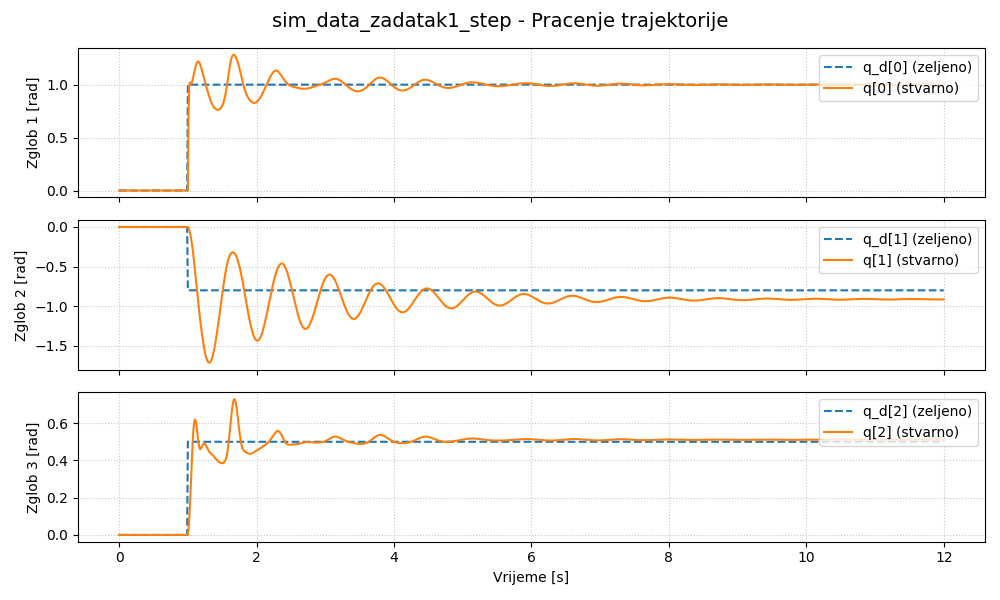
\includegraphics[width=0.9\textwidth]{../../src/data/sim_data_zadatak1_step_pozicije.png}
\caption{Zadatak 1 - Pozicije}
\vspace{0.5cm}
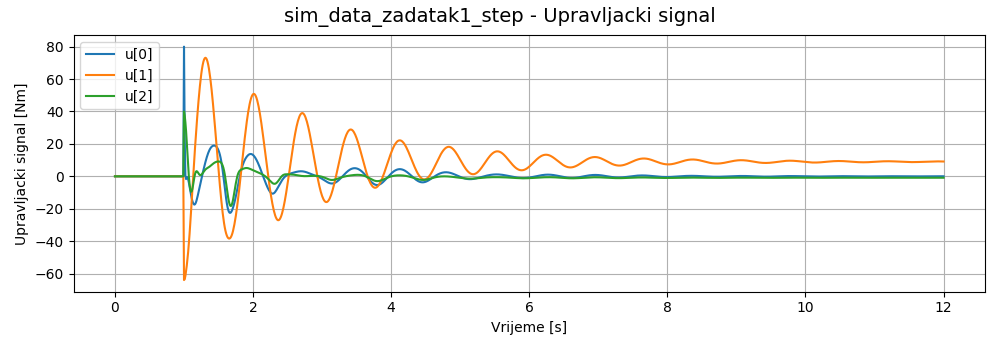
\includegraphics[width=0.9\textwidth]{../../src/data/sim_data_zadatak1_step_upravljanje.png}
\caption{Zadatak 1 - Upravljanje}
\end{figure}
\clearpage

\subsection{Zadatak 2: P regulator, sinusna referenca}
Zadržan je P regulator ($K_p = [80, 80, 80]$), no sada je cilj pratiti sinusoidnu referencu amplitude $A = [0.5, 0.4, 0.3]$ i frekvencije $f = 0.5$ Hz. Sustav kontinuirano kasni za referencom (zakašnjenje u fazi) i generira grešku (RMSE).

\begin{figure}[!ht]
\centering
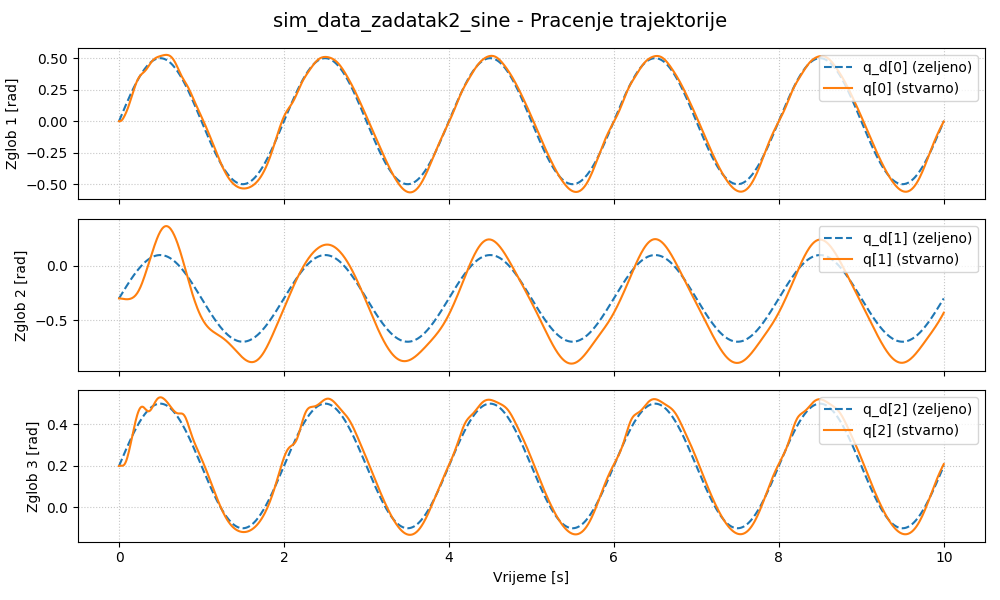
\includegraphics[width=0.9\textwidth]{../../src/data/sim_data_zadatak2_sine_pozicije.png}
\caption{Zadatak 2 - Pozicije}
\vspace{0.5cm}
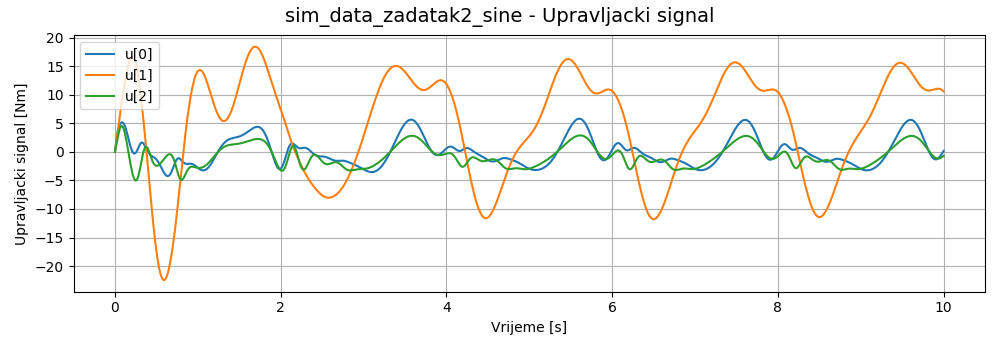
\includegraphics[width=0.9\textwidth]{../../src/data/sim_data_zadatak2_sine_upravljanje.png}
\caption{Zadatak 2 - Upravljanje}
\end{figure}
\clearpage

\subsection{Zadatak 3: PD regulator}
Kako bi se ublažile oscilacije primijećene u prvom zadatku, u sustav je dodan derivacijski član. Korištena je ista step referenca. Vrijednosti $K_d$ su ugađane eksperimentalno, no prevelike vrijednosti uzrokovale su numeričke nestabilnosti u diskretnom vremenu, pa su korištene vrlo blage vrijednosti $K_d = [0.1, 0.1, 0.1]$.

\begin{figure}[!ht]
\centering
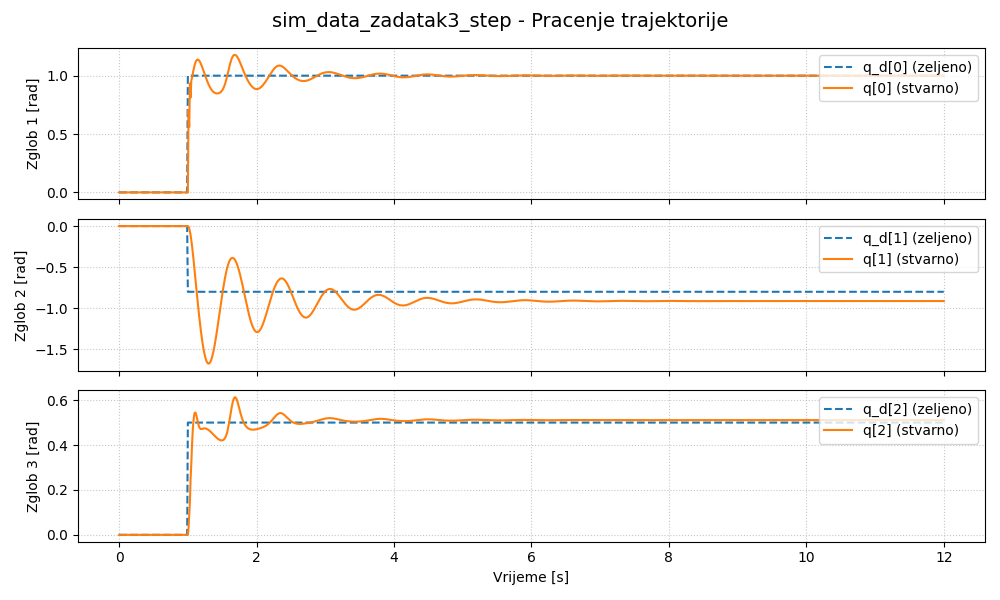
\includegraphics[width=0.9\textwidth]{../../src/data/sim_data_zadatak3_step_pozicije.png}
\caption{Zadatak 3 - Pozicije}
\vspace{0.5cm}
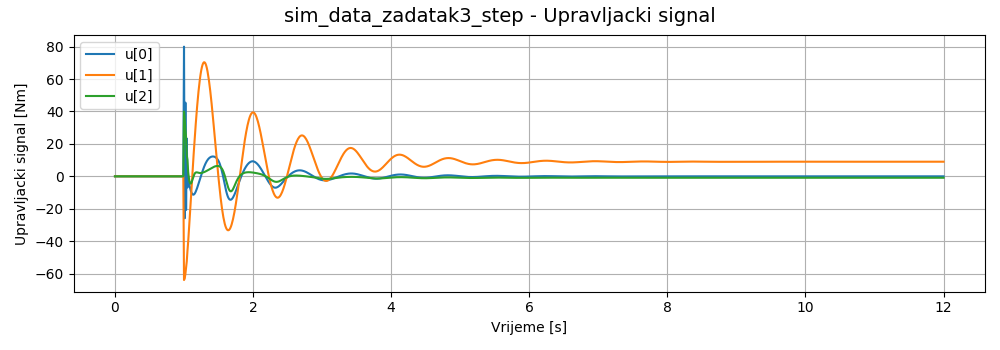
\includegraphics[width=0.9\textwidth]{../../src/data/sim_data_zadatak3_step_upravljanje.png}
\caption{Zadatak 3 - Upravljanje}
\end{figure}
\clearpage

\subsection{Zadatak 4: PD regulator uz smetnju (Disturbance)}
U ovom zadatku simulirana je statička smetnja od $5$ Nm koja djeluje na svaki zglob ($d = [5, 5, 5]$ Nm). Pojačanja su ostala ista kao u Zadatku 3. Može se primijetiti značajan porast stacionarne pogreške (steady-state error) jer PD regulator ne može integrativno kompenzirati statičku smetnju.

\begin{figure}[!ht]
\centering
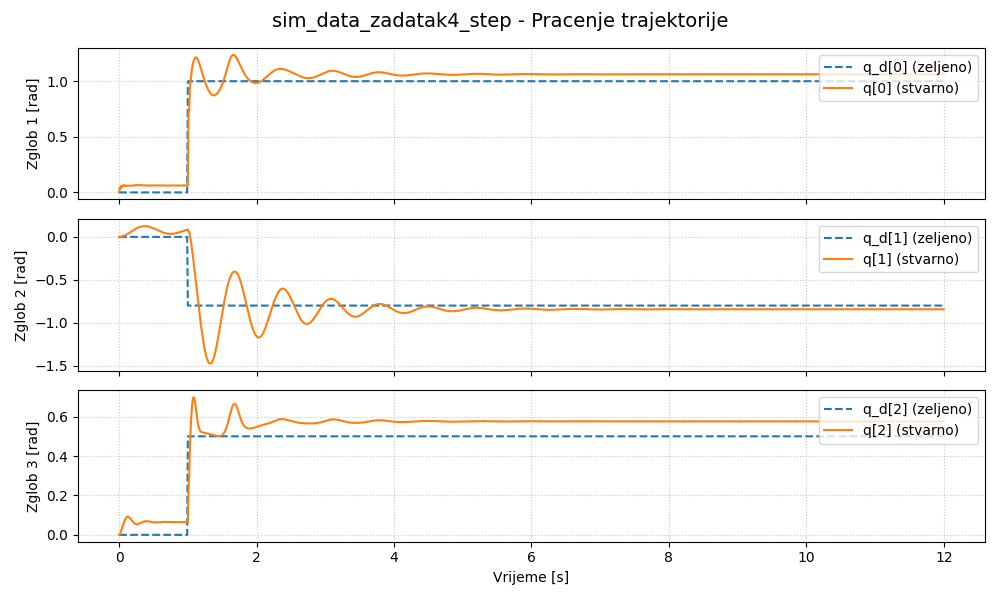
\includegraphics[width=0.9\textwidth]{../../src/data/sim_data_zadatak4_step_pozicije.png}
\caption{Zadatak 4 - Pozicije}
\vspace{0.5cm}
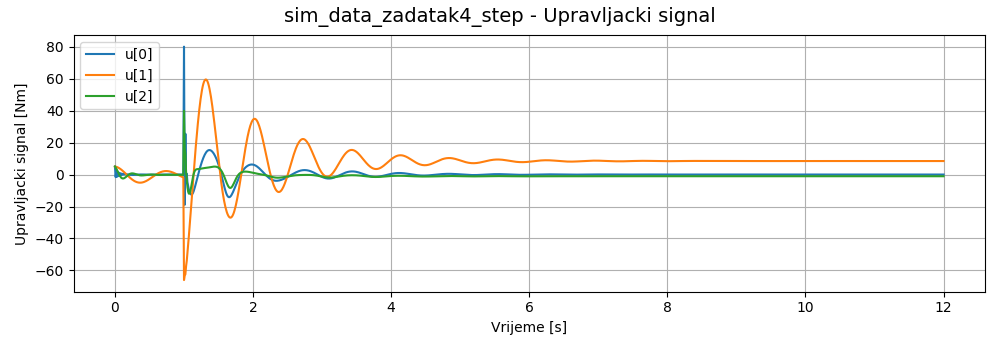
\includegraphics[width=0.9\textwidth]{../../src/data/sim_data_zadatak4_step_upravljanje.png}
\caption{Zadatak 4 - Upravljanje}
\end{figure}
\clearpage

\subsection{Zadatak 5: PID regulator}
Da bi se uklonila stacionarna pogreška uvedena smetnjom iz Zadatka 4, dodan je integralni član. $K_i$ je ugođen na $5.0$. Ovaj dodatak omogućava da se signal nakon skoka postepeno približi referenci, unatoč konstantnoj smetnji od $5$ Nm, što se jasno vidi na grafu pozicije u stacionarnom stanju.

\begin{figure}[!ht]
\centering
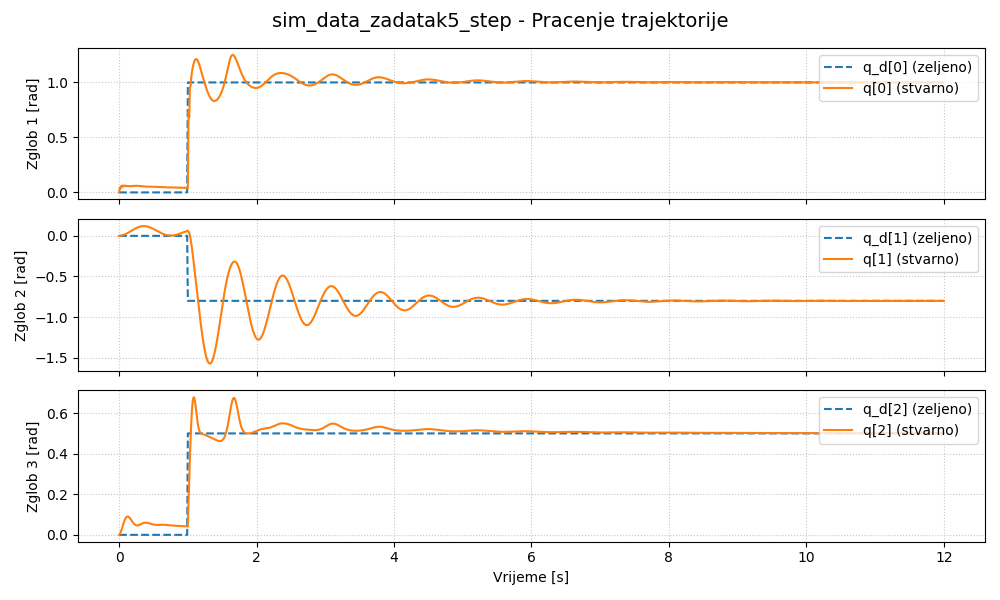
\includegraphics[width=0.9\textwidth]{../../src/data/sim_data_zadatak5_step_pozicije.png}
\caption{Zadatak 5 - Pozicije}
\vspace{0.5cm}
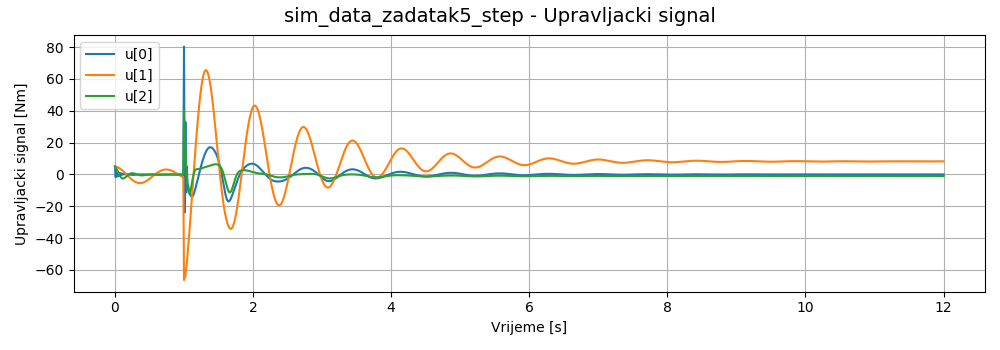
\includegraphics[width=0.9\textwidth]{../../src/data/sim_data_zadatak5_step_upravljanje.png}
\caption{Zadatak 5 - Upravljanje}
\end{figure}
\clearpage

\subsection{Zadatak 6: PID regulator uz mjerni šum}
U zadnjem eksperimentu ubačen je Gaussov šum ($\sigma = 0.02$ rad) u očitavanje pozicije iz senzora. Derivacijski član jako reagira na visokofrekventni šum, što uzrokuje da kontrolni signal ($u$) postane jako naboran (chattering).

\begin{figure}[!ht]
\centering
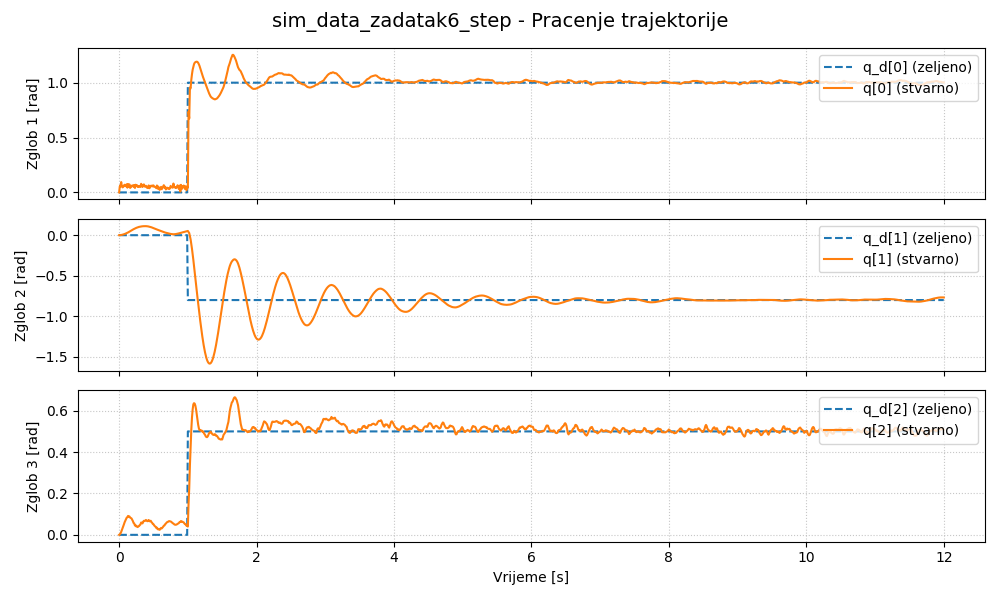
\includegraphics[width=0.9\textwidth]{../../src/data/sim_data_zadatak6_step_pozicije.png}
\caption{Zadatak 6 - Pozicije}
\vspace{0.5cm}
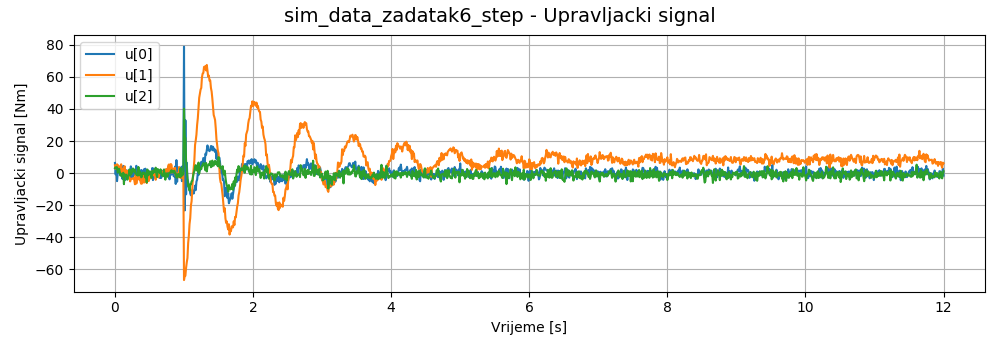
\includegraphics[width=0.9\textwidth]{../../src/data/sim_data_zadatak6_step_upravljanje.png}
\caption{Zadatak 6 - Upravljanje}
\end{figure}
\clearpage


\subsection{Zadatak 6.2: Optimizacija parametara uz mjerni šum}
U ovom zadatku izvršena je re-evaluacija i optimizacija svih parametara pomoću metode diferencijalne evolucije (stohastička optimizacija). Algoritam je minimizirao "cost" funkciju temeljenu na stacionarnoj pogrešci i vremenu smirivanja. Zanimljivo, algoritam je predložio značajno smanjenje proporcionalnog pojačanja ($K_p = 30.5$) što sprječava nepotrebno trzanje sustava uslijed šuma. S prigušenjem $K_d = 0.5$ i sporijim integralnim članom $K_i = 11$, sustav postiže manji \textit{steady-state error} i brže vrijeme smirivanja na najtežem zglobu (zglob 2) u odnosu na Zadatak 6.

\begin{figure}[!ht]
\centering
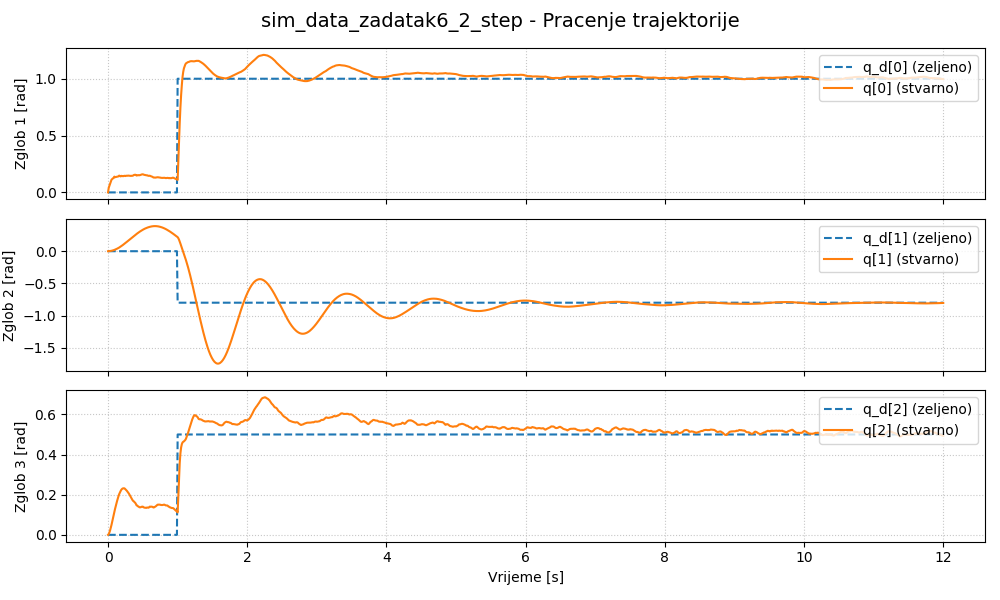
\includegraphics[width=0.9\textwidth]{../../src/data/sim_data_zadatak6_2_step_pozicije.png}
\caption{Zadatak 6.2 - Pozicije (Optimizirano)}
\vspace{0.5cm}
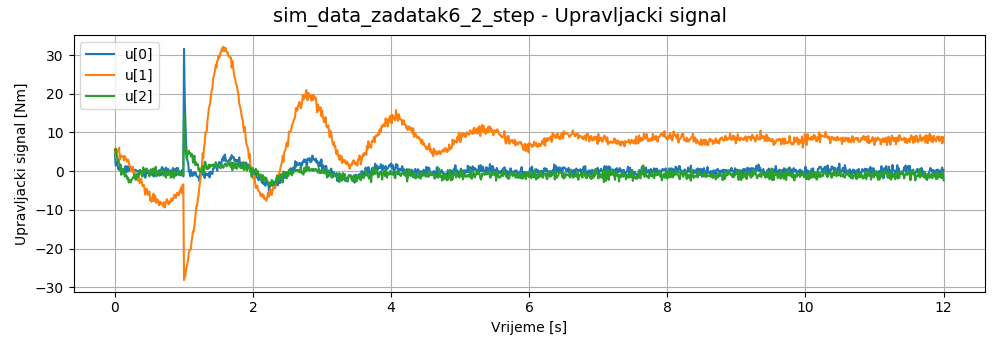
\includegraphics[width=0.9\textwidth]{../../src/data/sim_data_zadatak6_2_step_upravljanje.png}
\caption{Zadatak 6.2 - Upravljanje (Optimizirano)}
\end{figure}
\clearpage

\section{USPOREDBA I METRIKE}

U donjoj tablici nalazi se zbirna usporedba izračunatih metrika za sve provedene eksperimente uz step referencu. Vremena smirivanja (Settling Time) za sve eksperimente su zaustavljena blizu maksimalnog trajanja od 12.0 sekundi, što indicira da se sustav nije do kraja smirio unutar pojasne širine od $\pm 2\%$ u zadanom trajanju, ili oscilira jako dugo.

\begin{table}[!ht]
\centering
\caption{Usporedba metrika}
\resizebox{\textwidth}{!}{
\begin{tabular}{|l|l|l|l|l|l|l|l|l|l|}
\hline
\textbf{Joint} & \textbf{Zadatak} & \textbf{Ref} & \textbf{Kp} & \textbf{Kd} & \textbf{Ki} & \textbf{Overshoot [\%]} & \textbf{Settling Time [s]} & \textbf{SS Error [rad]} & \textbf{RMSE [rad]} \\ \hline
1     & 1. P    & Step & 80 & 0   & 0  & 28.20         & 4.190             & 0.000          & -          \\ \hline
2     & 1. P    & Step & 80 & 0   & 0  & 114.29        & 7.100             & 0.114          & -          \\ \hline
3     & 1. P    & Step & 80 & 0   & 0  & 45.74         & 3.810             & -0.011         & -          \\ \hline
1     & 2. P    & Sine & 80 & 0   & 0  & -             & -                 & -              & 0.031      \\ \hline
2     & 2. P    & Sine & 80 & 0   & 0  & -             & -                 & -              & 0.130      \\ \hline
3     & 2. P    & Sine & 80 & 0   & 0  & -             & -                 & -              & 0.026      \\ \hline
1     & 3. PD   & Step & 80 & 0.7 & 0  & 17.82         & 2.470             & 0.000          & -          \\ \hline
2     & 3. PD   & Step & 80 & 0.7 & 0  & 109.34        & 4.260             & 0.113          & -          \\ \hline
3     & 3. PD   & Step & 80 & 0.7 & 0  & 22.50         & 1.790             & -0.011         & -          \\ \hline
1     & 4. PD+D & Step & 80 & 0.7 & 0  & 23.68         & 2.510             & -0.062         & -          \\ \hline
2     & 4. PD+D & Step & 80 & 0.7 & 0  & 84.52         & 4.230             & 0.043          & -          \\ \hline
3     & 4. PD+D & Step & 80 & 0.7 & 0  & 39.58         & 2.130             & -0.076         & -          \\ \hline
1     & 5. PID+D& Step & 80 & 0.7 & 35 & 25.07         & 3.610             & 0.000          & -          \\ \hline
2     & 5. PID+D& Step & 80 & 0.7 & 35 & 96.62         & 6.050             & 0.001          & -          \\ \hline
3     & 5. PID+D& Step & 80 & 0.7 & 35 & 35.58         & 4.970             & -0.001         & -          \\ \hline
1     & 6. PID+D+N& Step & 80 & 0.7 & 35 & 25.34         & 10.690            & -0.003         & -          \\ \hline
2     & 6. PID+D+N& Step & 80 & 0.7 & 35 & 98.00         & 10.840            & -0.032         & -          \\ \hline
3     & 6. PID+D+N& Step & 80 & 0.7 & 35 & 32.96         & 10.790            & -0.008         & -          \\ \hline
1     & 6.2. Opt & Step & 30.5 & 0.5 & 11 & 21.00         & 10.730            & 0.003          & -          \\ \hline
2     & 6.2. Opt & Step & 30.5 & 0.5 & 11 & 118.30        & 9.310             & 0.003          & -          \\ \hline
3     & 6.2. Opt & Step & 30.5 & 0.5 & 11 & 37.03         & 10.910            & 0.005          & -          \\ \hline
\end{tabular}
}
\end{table}

\section{ZAKLJUČAK}
Provedeni eksperimenti na modelu 3DOF robotske ruke jasno i praktično demonstriraju uloge pojedinih članova PID regulatora. Proporcionalni (P) član osigurava osnovnu brzinu odziva i usmjerava sustav prema ciljnoj poziciji, ali ne može samostalno eliminirati stacionarnu pogrešku te često uzrokuje prebačaje. Dodavanjem derivacijskog (D) člana uvodi se prigušenje, smanjujući oscilacije i stabilizirajući sustav, no njegova je primjena ograničena izrazitom osjetljivošću na mjerni šum. Konačno, uvođenjem integralnog (I) člana omogućeno je akumuliranje pogreške kroz vrijeme, što je ključno za potpuno poništavanje stacionarne pogreške uzrokovane konstantnim vanjskim smetnjama. Eksperimentalnim putem odabrane su vrijdnosti pojačanja, te smo uspjeli postići brz i precizan odziv sustava u uvjetima šuma i vanjskih poremećaja.

\end{document}
